\documentclass[UTF-8, a4paper, 10pt]{article}

\usepackage{xeCJK}
\usepackage{graphicx}
\graphicspath{{figure/}}
\usepackage[unicode]{hyperref}
\hypersetup{colorlinks=true,linkcolor=black}
\usepackage{cite}
\usepackage{indentfirst}
\usepackage{amsmath}
\numberwithin{equation}{section}
\usepackage{listings}
\usepackage{xcolor}
\usepackage{fontspec}
\usepackage{courier}
\usepackage{booktabs}
\usepackage{tikz-timing}

\lstset{
    basicstyle=\scriptsize\ttfamily,
    numbers=left,                                        % 在左侧显示行号
    keywordstyle=\color[RGB]{40,40,255},                 % 设定关键字颜色
    frame=trbl,
    numberstyle=\scriptsize\color{darkgray},           % 设定行号格式
    commentstyle=\it\color[RGB]{0,96,96},                % 设置代码注释的格式
    stringstyle=\ttfamily\slshape\color[RGB]{128,0,0},   % 设置字符串格式
    showstringspaces=false,                              % 不显示字符串中的空格
    language=python,                                     % 设置语言
}


\linespread{1.0}
\setlength{\parskip}{0.5\baselineskip}

\makeatletter
\let\@afterindentfalse\@afterindenttrue
\@afterindenttrue
\makeatother
\setlength{\parindent}{2em}

\addtolength{\topmargin}{-70pt}
\setlength{\oddsidemargin}{0.63cm}
\setlength{\evensidemargin}{\oddsidemargin}
\setlength{\textwidth}{15.66cm}
\setlength{\textheight}{25.00cm}

\newcommand{\chuhao}{\fontsize{42pt}{\baselineskip}\selectfont}
\newcommand{\xiaochuhao}{\fontsize{36pt}{\baselineskip}\selectfont}
\newcommand{\yihao}{\fontsize{28pt}{\baselineskip}\selectfont}
\newcommand{\erhao}{\fontsize{21pt}{\baselineskip}\selectfont}
\newcommand{\xiaoerhao}{\fontsize{18pt}{\baselineskip}\selectfont}
\newcommand{\sanhao}{\fontsize{15.75pt}{\baselineskip}\selectfont}
\newcommand{\sihao}{\fontsize{14pt}{\baselineskip}\selectfont}
\newcommand{\xiaosihao}{\fontsize{12pt}{\baselineskip}\selectfont}
\newcommand{\wuhao}{\fontsize{10.5pt}{\baselineskip}\selectfont}
\newcommand{\xiaowuhao}{\fontsize{9pt}{\baselineskip}\selectfont}
\newcommand{\liuhao}{\fontsize{7.875pt}{\baselineskip}\selectfont}
\newcommand{\qihao}{\fontsize{5.25pt}{\baselineskip}\selectfont}

\begin{document}

\begin{titlepage}
    \begin{center}
    \phantom{Start!}
	\vspace{2cm}
	
\includegraphics[width=350pt]{HUST.pdf} \\
    \vspace{1cm}
     \center{
       	  \textbf{\yihao 实\quad 验\quad 报\quad 告}\\
       	  \vspace{0.5cm}
          \textbf{\sanhao (2017 / 2018学年\quad 第2学期)}
      }
      \vspace{2.5cm}
      \begin{table}[!hbp]
      \centering
      \renewcommand\arraystretch{1.5}
     	\begin{tabular}{|c|c|}
     		\hline
     		课程名称 & 机器学习导论 \\
     		\hline
     		实验名称 & ~~~~~~Support vector machine~~~~~~ \\
     		\hline
     		实验时间&\multicolumn{1}{c|}{2018年6月15日}\\
     		\hline
     		指导教师 & 王邦 \\
     		\hline
     		\end{tabular}     		
       \end{table}
       \vspace{2cm}
      \begin{table}[htbp]
      \centering
      \renewcommand\arraystretch{1.5}
     	\begin{tabular}{|c|c|c|c|}
     		\hline
            \qquad ~~姓名~~~~~  & \qquad ~~游浩然~~~~~  & \qquad 学号~~~~~ & \qquad U201515429~~~~~ \\
     		\hline
     		\end{tabular}
       \end{table}
       \date{2018年5月29日}
     \end{center}
\end{titlepage}

\section{问题重述}
\begin{itemize}
  \item 给定数据集(文件 data1\_Task.mat)如下图所示, 参考Demo 1和Demo 2 , 编程实现一个高斯核SVM进行分类。输出训练参数C, sigma分别取0.01, 0.03, 0.1, 0.3, 1, 3, 10, 30时(共64组参数组合)的训练集上的准确率。
  \item 编程实现一个垃圾邮件SVM线性分类器,分别在训练集和测试集上计算准确率。
        训练数据文件:spamTrain.mat,要求导入数据时输出样本数和特征维度。
        测试数据文件:spamTest.mat,要求导入数据时输出样本数和特征维度。

\end{itemize}

\section{Python Code for SVM}
\subsection{SVM}
\begin{lstlisting}[language=python]
# -*- coding: utf-8 -*-
"""
@author : Haoran You

"""
import time
import numpy as np
import matplotlib.pyplot as plt

class SVM():
    def name(self):
        return 'svm classifier'

    def svmTrain_SMO(self, X, y, C, kernal_function='linear', tol=1e-3, max_iter=5, **kargs):
        """
        :param X:
        :param y:
        :param C: punishment coefficient
        :param kernal_function: type of kernal function; for nonlinear function, input K directly
        :param tol: error-tolerant rate
        :param max_iter: maximum iterations
        :param kargs:
        :return: model['kernelFunction]: kernal function type
        :return: model['X']: support vector
        :return: model['y']: label
        :return: model['alpha']: corresponding lagrange parameters
        :return: model['w'], model['b']: model parameters
        """
        start_time = time.clock()

        m, n = X.shape
        X = np.mat(X)
        y = np.mat(y, dtype='float64')
        y[np.where(y==0)] = -1
        alpha = np.mat(np.zeros((m, 1)))
        b = 0.0
        E = np.mat(np.zeros((m, 1)))
        iters = 0
        eta = 0.0
        L = 0.0
        H = 0.0

        if kernal_function == 'linear':
            K = X*X.T
        elif kernal_function == 'gaussian':
            K = kargs['K_matrix']
        else:
            print('Kernal Error')
            return None

        print('Training ...', end='')
        dots = 12
        while iters < max_iter:
            num_changed_alpha = 0
            for i in range(m):
                E[i] = b + np.sum(np.multiply(np.multiply(alpha, y), K[:, i])) - y[i]
                if (y[i]*E[i] < -tol and alpha[i] < C) or (y[i]*E[i] > tol and alpha[i] > 0):
                    j = np.random.randint(m)
                    while j == i:
                        j = np.random.randint(m)
                    E[j] = b + np.sum(np.multiply(np.multiply(alpha, y), K[:, j])) - y[j]

                    alpha_i_old = alpha[i].copy()
                    alpha_j_old = alpha[j].copy()

                    if y[i] == y[j]:
                        L = max(0, alpha[j] + alpha[i] - C)
                        H = min(C, alpha[j] + alpha[i])
                    else:
                        L = max(0, alpha[j] - alpha[i])
                        H = min(C, C + alpha[j] - alpha[i])

                    if L == H:
                        continue

                    eta = 2 * K[i, j] - K[i, i] - K[j, j]
                    if eta >= 0:
                        continue

                    alpha[j] = alpha[j] - (y[j]*(E[i] - E[j])) / eta
                    alpha[j] = min(H, alpha[j])
                    alpha[j] = max(L, alpha[j])

                    if abs(alpha[j] - alpha_j_old) < tol:
                        alpha[j] = alpha_j_old
                        continue

                    alpha[i] = alpha[i] + y[i] * y[j] * (alpha_j_old - alpha[j])

                    b1 = b - E[i]\
                     - y[i] * (alpha[i] - alpha_i_old) * K[i, j]\
                     - y[j] * (alpha[j] - alpha_j_old) * K[i, j]

                    b2 = b - E[j]\
                     - y[i] * (alpha[i] - alpha_i_old) * K[i, j]\
                     - y[j] * (alpha[j] - alpha_j_old) * K[i, j]

                    if (0 < alpha[i] and alpha[i] < C):
                        b = b1
                    elif (0 < alpha[j] and alpha[j] < C):
                        b = b2
                    else:
                        b = (b1 + b2) / 2.0

                    num_changed_alpha = num_changed_alpha + 1

            if num_changed_alpha == 0:
                iters = iters + 1
            else:
                iters = 0

            print('.', end='')
            dots = dots + 1
            if dots > 78:
                dots = 0
                print()

        print('Done', end='')
        end_time = time.clock()
        print('( ' + str(end_time - start_time) + 's )')
        print()

        idx = np.where(alpha > 0)
        model = {
            'X': X[idx[0], :],
            'y': y[idx],
            'kernelFunction': str(kernal_function),
            'b': b,
            'alpha':alpha[idx],
            'w': (np.multiply(alpha, y).T * X).T
        }
        return model

    def visualizeBoundaryLinear(self, X, y, model, title=None):
        fig = plt.figure()
        ax = fig.add_subplot(111)

        w = model['w']
        b = model['b']
        xp = np.linspace(min(X[:, 0]), max(X[:, 0]), 100)
        yp = np.squeeze(np.array(- (w[0] * xp + b) / w[1]))

        ax.plot(xp, yp)

        # scatter
        X_pos = []
        X_neg = []

        sampleArray = np.concatenate((X, y), axis=1)
        for array in list(sampleArray):
            if array[-1]:
                X_pos.append(array)
            else:
                X_neg.append(array)

        X_pos = np.array(X_pos)
        X_neg = np.array(X_neg)

        if title: ax.set_title(title)

        pos = plt.scatter(X_pos[:, 0], X_pos[:, 1], marker='+', c='b')
        neg = plt.scatter(X_neg[:, 0], X_neg[:, 1], marker='o', c='y')

        plt.legend((pos, neg), ('postive', 'negtive'), loc=2)

        plt.show()

    def gaussianKernelSub(self, x1, x2, sigma):
        X1 = np.mat(x1).reshape(-1, 1)
        X2 = np.mat(x2).reshape(-1, 1)
        n = -(x1-x2).T * (x1 - x2) / (2*sigma**2)
        return np.exp(n)

    def gaussianKernel(self, X, sigma):
        start = time.clock()

        print('GaussianKernel Computing ...', end='')
        m = X.shape[0]
        X = np.mat(X)
        K = np.mat(np.zeros((m, m)))
        dots = 280
        for i in range(m):
            if dots % 10 == 0: print('.', end='')
            dots = dots + 1
            if dots > 780:
                dots = 0
                print()
            for j in range(m):
                K[i, j] = self.gaussianKernelSub(X[i, :].T, X[j, :].T, sigma)
                K[j, i] = K[i, j].copy()

        print('Done', end='')
        end = time.clock()
        print('( ' + str(end - start) + 's )')
        print()
        return K

    def svmPredict(self, model, X, *arg):
        m = X.shape[0]
        p = np.mat(np.zeros((m, 1)))
        pred = np.mat(np.zeros((m, 1)))

        if model['kernelFunction'] == 'linear':
            p = X * model['w'] + model['b']
        else:
            for i in range(m):
                prediction = 0
                for j in range(model['X'].shape[0]):
                    prediction += model['alpha'][:, j] * model['y'][:, j] * \
                                  self.gaussianKernelSub(X[i, :].T, model['X'][j, :].T, *arg)

                p[i] = prediction + model['b']

        pred[np.where(p >= 0)] = 1
        pred[np.where(p < 0)] = 0

        return pred

    def visualizeBoundaryGaussian(self, X, y, model, sigma):
        fig = plt.figure()
        ax = fig.add_subplot(111)

        x1plot = np.linspace(min(X[:, 0]), max(X[:, 0]), 100)
        x2plot = np.linspace(min(X[:, 1]), max(X[:, 1]), 100)
        X1, X2 = np.meshgrid(x1plot, x2plot)
        X1 = np.mat(X1)
        X2 = np.mat(X2)
        vals = np.mat(np.zeros(X1.shape))

        print('Predicting ...', end='')
        dots = 14
        for i in range(X1.shape[1]):
            print('.', end='')
            dots += 1
            if dots == 78:
                dots = 0
                print()
            this_X = np.concatenate((X1[:, i], X2[:, i]), axis=1)
            vals[:, i] = self.svmPredict(model, this_X, sigma)
        print('Done')

        ax.contour(X1, X2, vals, colors='black')
        # scatter
        X_pos = []
        X_neg = []

        sampleArray = np.concatenate((X, y), axis=1)
        for array in list(sampleArray):
            if array[-1]:
                X_pos.append(array)
            else:
                X_neg.append(array)

        X_pos = np.array(X_pos)
        X_neg = np.array(X_neg)

        pos = plt.scatter(X_pos[:, 0], X_pos[:, 1], marker='+', c='b')
        neg = plt.scatter(X_neg[:, 0], X_neg[:, 1], marker='o', c='y')

        plt.legend((pos, neg), ('postive', 'negtive'), loc=2)

        plt.show()

\end{lstlisting}
\subsection{data}
\begin{lstlisting}[language=python]
# -*- coding: utf-8 -*-
"""
@author : Haoran You

"""
from scipy.io import loadmat
import numpy as np
import matplotlib.pyplot as plt

def loadData(filename):
    dataDict = loadmat(filename)
    return dataDict['X'], dataDict['y']

def plotData(X, y, title=None):
    X_pos = []
    X_neg = []

    sampleArray = np.concatenate((X, y), axis=1)
    for array in list(sampleArray):
        if array[-1]:
            X_pos.append(array)
        else:
            X_neg.append(array)

    X_pos = np.array(X_pos)
    X_neg = np.array(X_neg)

    fig = plt.figure()

    ax = fig.add_subplot(111)

    if title: ax.set_title(title)

    pos = plt.scatter(X_pos[:, 0], X_pos[:, 1], marker='+', c='b')
    neg = plt.scatter(X_neg[:, 0], X_neg[:, 1], marker='o', c='y')

    plt.legend((pos, neg), ('postive', 'negtive'), loc=2)

    plt.show()

\end{lstlisting}
\newpage
\subsection{Main}
\begin{lstlisting}[language=python]
# -*- coding: utf-8 -*-
"""
@author : Haoran You

"""
import os
from data import *
from SVM import SVM

file_path = os.getcwd()

def Task1():
    # load and visulize data
    svm = SVM()
    print('Loading and Visualizing Data ...')
    X, y = loadData(file_path + '\data1_Task.mat')
    plotData(X, y, title='Task 1')

    print('Program paused. Press enter to continue.')
    input()

    # Training
    print('Training SVM with RBF kernel ...')
    param = [0.01, 0.03, 0.1, 0.3, 1, 3, 10, 30]
    acc = []
    for C in param:
        for sigma in param:
            model = svm.svmTrain_SMO(X, y, C, kernal_function='gaussian', K_matrix=svm.gaussianKernel(X, sigma))
            pred = svm.svmPredict(model, np.mat(X), sigma)
            acc.append(1 - np.sum(abs(pred - y)) / len(y))
    print(acc)
    f = open('results.txt', 'a+')
    f.write('sigma\t%.3f\t%.3f\t%.3f\t%.3f\t%.3f\t%.3f\t%.3f\t%.3f\nC\n' \
            % (0.010, 0.030, 0.100, 0.300, 1.000, 3.000, 10.000, 30.000))
    count = 0
    for i in range(len(param)):
        content = '%.3f\t' % param[i]
        for j in range(len(param)):
            content += '%.3f\t' % acc[count]
            count += 1
        content += '\n'
        f.write(content)
    f.close()

    # results visualizing
    # print('Results visualizing ...')
    # svm.visualizeBoundaryGaussian(X, y, model, sigma)

def Task2():
    # load data
    print('Loading data ...')
    X_train, y_train = loadData(file_path + '\spamTrain.mat')
    X_test, y_test = loadData(file_path + '\spamTest.mat')
    # plotData(X_train, y_train, title='Task 2')

    print('Program paused. Press enter to continue.\n')
    input()

    # trainging
    svm = SVM()
    print('Number of samples: {}'.format(X_train.shape[0]))
    print('Number of features: {}'.format(X_train.shape[1]))
    print('Training Linear SVM ...')
    C = 1; sigma = 0.01;
    model = svm.svmTrain_SMO(X_train, y_train, C, max_iter=20)
    pred_train = svm.svmPredict(model, np.mat(X_train), sigma)
    acc_train = 1 - abs(np.sum(pred_train - y_train)) / len(y_train)
    print('Train accuracy: {}'.format(acc_train))

    # test
    print('Number of samples: {}'.format(X_test.shape[0]))
    print('Number of features: {}'.format(X_test.shape[1]))
    pred_test = svm.svmPredict(model, np.mat(X_test), sigma)
    acc_test = 1 - abs(np.sum(pred_test - y_test)) / len(y_test)
    print('Test accuracy: {}'.format(acc_test))

if __name__ == '__main__':
    Task2()
\end{lstlisting}

\newpage
\subsection{Results}
\subsubsection{Task1}
% Table generated by Excel2LaTeX from sheet 'Sheet1'
\begin{table}[htbp]
  \centering
  \caption{Results for different parameters C \& sigma}
    \begin{tabular}{ccccccccc}
    \toprule
    sigma & 0.01  & 0.03  & 0.1   & 0.3   & 1     & 3     & 10    & 30 \\
    C     &       &       &       &       &       &       &       &  \\
    \midrule
    0.01  & 0.498 & 0.498 & 0.502 & 0.502 & 0.502 & 0.498 & 0.502 & 0.502 \\
    0.03  & 0.502 & 0.502 & 0.502 & 0.867 & 0.502 & 0.498 & 0.834 & 0.498 \\
    0.1   & 0.498 & 0.502 & 0.943 & 0.872 & 0.834 & 0.81  & 0.815 & 0.81 \\
    0.3   & 0.502 & 0.981 & 0.948 & 0.905 & 0.867 & 0.81  & 0.498 & 0.502 \\
    1     & 1     & 0.995 & 0.948 & 0.934 & 0.905 & 0.848 & 0.815 & 0.829 \\
    3     & 1     & 1     & 0.943 & 0.943 & 0.915 & 0.863 & 0.825 & 0.502 \\
    10    & 1     & 1     & 0.962 & 0.934 & 0.929 & 0.9   & 0.848 & 0.815 \\
    30    & 1     & 1     & 0.948 & 0.943 & 0.924 & 0.919 & 0.867 & 0.791 \\
    \bottomrule
    \end{tabular}%
  \label{tab:addlabel}%
\end{table}%

\begin{figure}[!htbp]
  \centering
  \begin{minipage}[t]{7.5cm}
    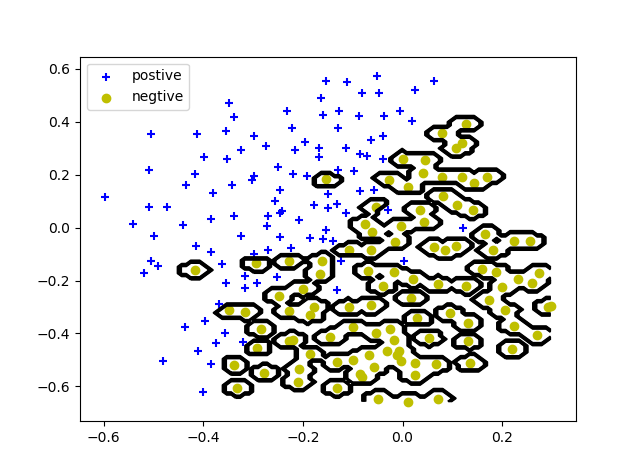
\includegraphics[width=7cm]{figure1.png}
    \centerline{C = 1 \& sigma = 0.01}
  \end{minipage}
  \begin{minipage}[t]{7.5cm}
    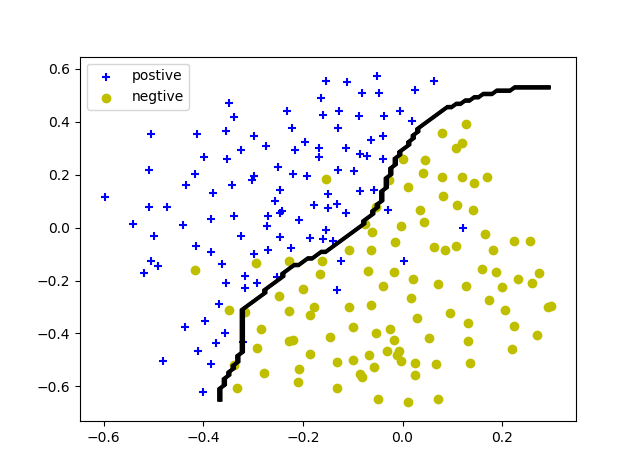
\includegraphics[width=7cm]{figure2.png}
    \centerline{C = 1 \& sigma = 0.1}
  \end{minipage}
  \caption{Boundary Visualization}\label{svm}
\end{figure}
\subsubsection{Task2}
\begin{itemize}
  \item Train accuracy: 0.98775
    \begin{itemize}
      \item Number of samples: 4000
      \item Number of features: 1899
    \end{itemize}
  \item Test accuracy: 0.982
    \begin{itemize}
      \item Number of samples: 1000
      \item Number of features: 1899
    \end{itemize}
\end{itemize}
\end{document} 